\section{Agent-Coordinated Task-Level Operation}
\label{sec:closed-loop-operation}

\begin{figure*}[!t]
\centering
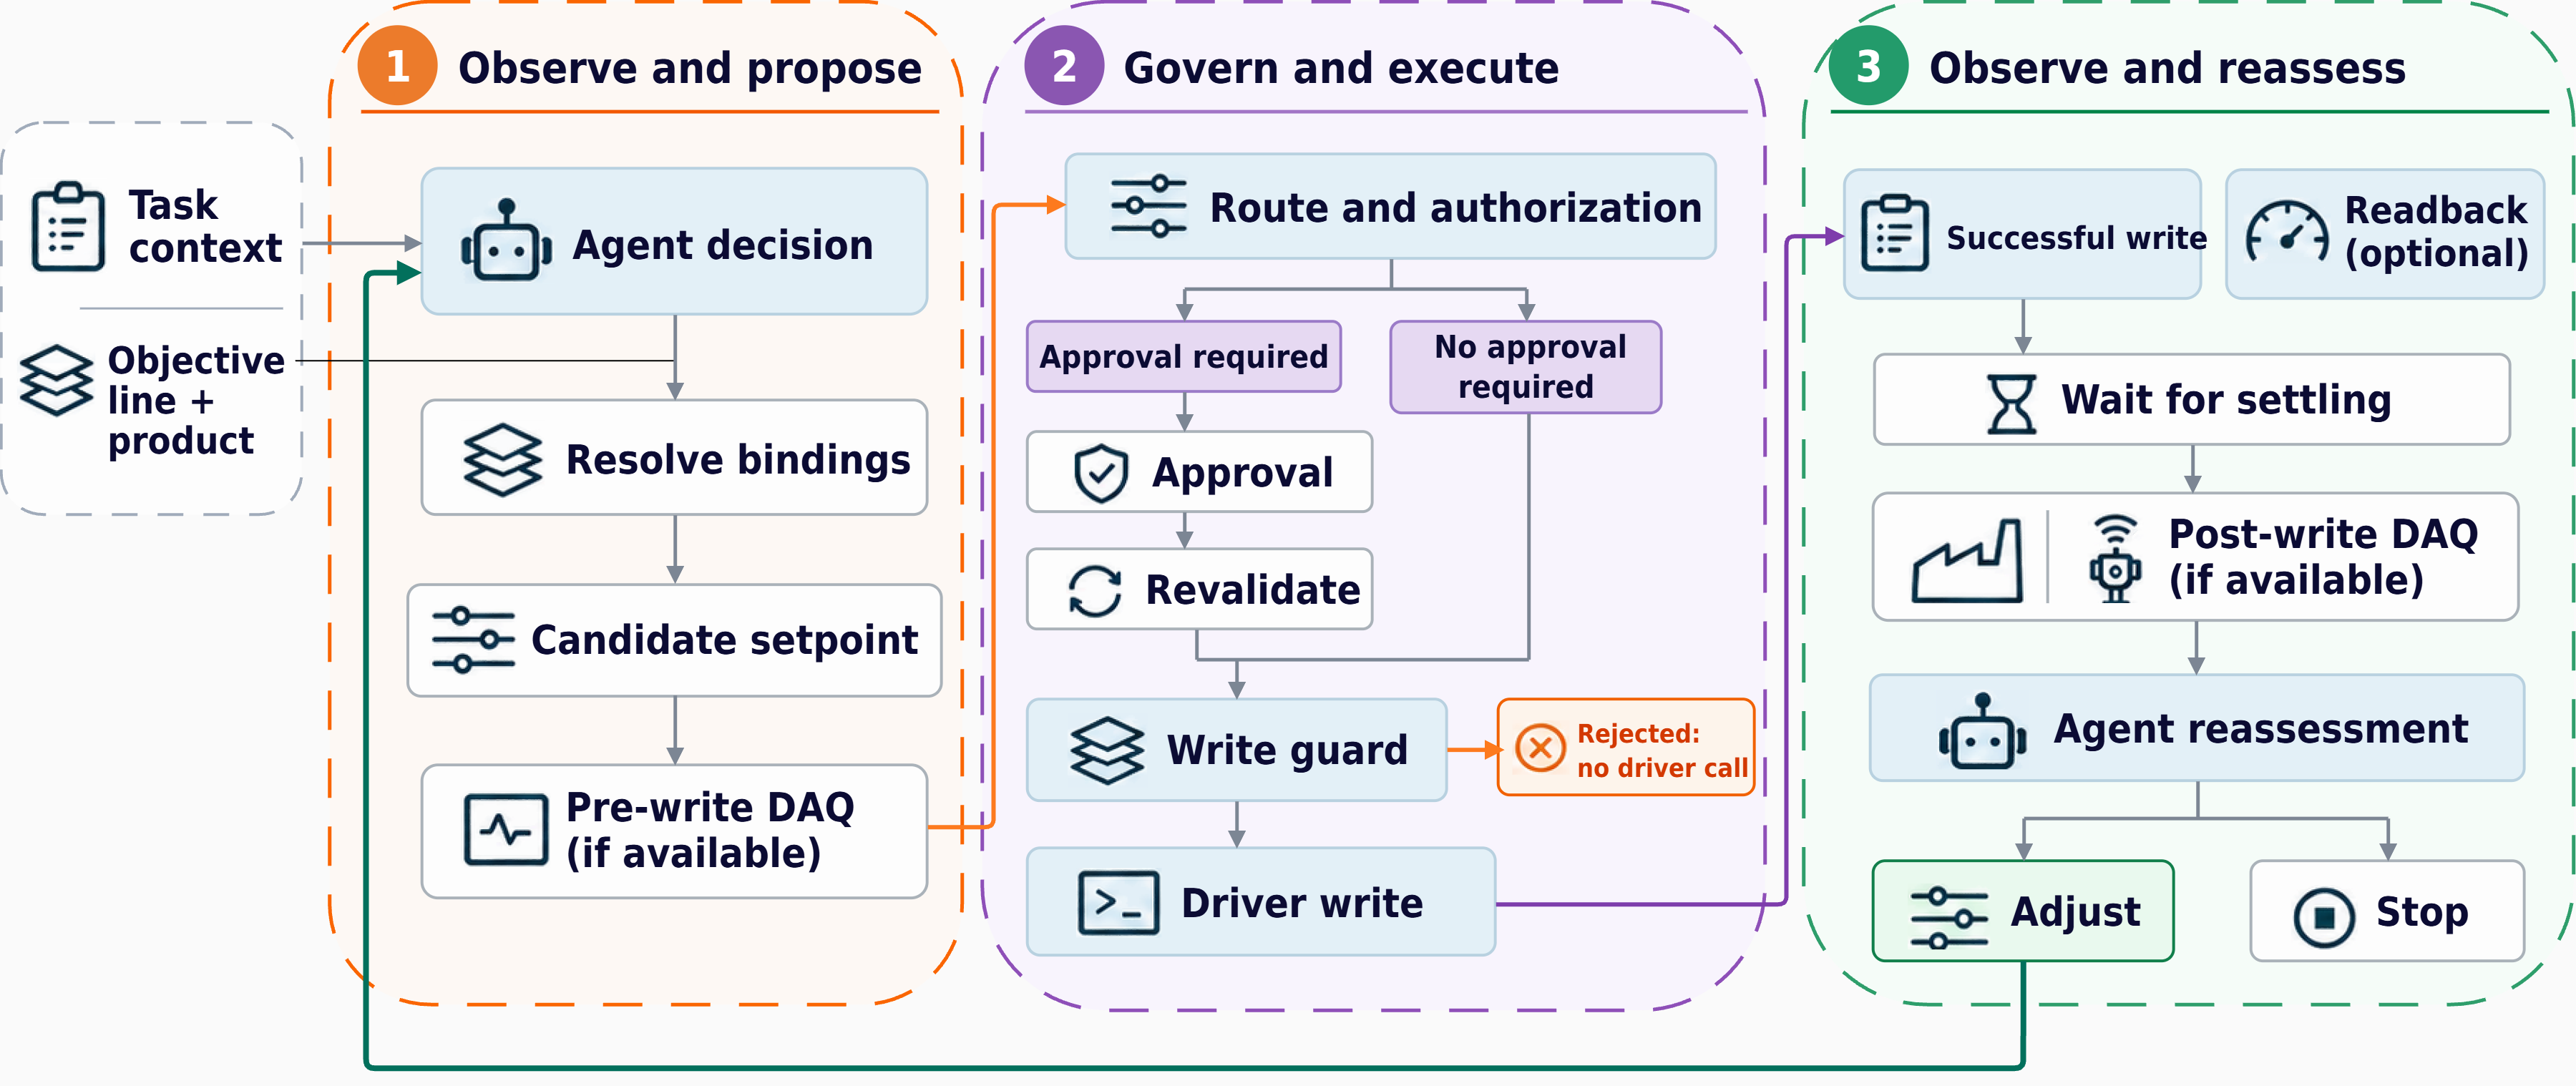
\includegraphics[width=\textwidth]{resources/fig3.png}
\caption{Conceptual agent-mediated online acquisition and control loop: the agent acquires observations, analyzes the objective gap, proposes a setpoint, and the write path applies route-dependent checks before controlled dispatch. The agent may reassess returned evidence before another adjustment or stopping. Observations available before the agent decision are not separately shown; pre-write DAQ is a subsequent optional read. Requests requiring approval proceed to route-specific revalidation only after approval; requests denied before dispatch do not reach the driver. The approval-denial branch is omitted. Routes without required approval bypass the approval wait but remain subject to applicable dispatch, authorization, and write-guard checks. A driver error may leave device state uncertain. Command outcomes and optional readback are distinct from later DAQ observations; the readback box is schematic.}
\label{fig:agent-loop}
\end{figure*}

A task supplies an objective and production context. The agent can call \texttt{daq\_query} to read recent timestamped samples collected by the DAQ service. The call queries stored observations rather than polling the device itself. The control node comes from \texttt{control\_node\_id} or a configured binding; the DAQ target comes from an explicit ID or a DAQ binding. Observations inform a typed adjustment but do not authorize it. Fig.~\ref{fig:agent-loop} shows the intended iteration, not a measurement trace.

In goal mode, a lead agent may decompose the objective and dispatch worker subtasks. For an exploration step, the responsible agent may invoke \texttt{optimization\_explore}, which resolves the DAQ target, checks bindings, and submits a candidate before device I/O.

The operation resolves the profile and control binding, then reads the stored value as $u_0$; this is not necessarily a fresh readback. The agent combines this state with its objective and direction. If direction is omitted, the operation defaults upward; otherwise $s\in\{-1,+1\}$. For a step $\Delta u$, it forms
\begin{equation}
 u^{*}=\operatorname{clip}\!\left(u_0+s\Delta u,\,u_{\min},\,u_{\max}\right).
 \label{eq:optimization-candidate}
\end{equation}
In Eq.~(\ref{eq:optimization-candidate}), configured tuning bounds take precedence; node bounds are used otherwise. The effective step is selected in this order: an explicit argument, the binding's tuning step, the scene's maximum step, or one twentieth of the node range.

The operation checks DAQ target visibility before admitting the intent. The available implementation also contains identifiability and model--ontology gates; the archived trials do not establish whether these gates were deployed or exercised. If the checks pass, the operation attempts a pre-write DAQ read, whose mean may be unavailable.

A valid candidate enters the governed single-node write path in Algorithm~1. A pre-dispatch denial stops the request before any driver call. A driver-stage error, by contrast, may occur after dispatch has begun, so status alone cannot establish whether the device changed; state must be read and reconciled before retrying.

After a successful write, the operation waits 10--300~s (45~s by default) and attempts a post-write DAQ read. The available anchored-window implementation uses $[t_0-\tau,t_0]$ and $[t_0,t_1]$, where $t_0$ precedes the governed write call and $t_1$ is the follow-up query time. The second window can include time spent awaiting approval before dispatch, so a difference between window means does not establish a write effect. Earlier code used trailing 45-s windows.

The exploration record stores the target, the step, the available DAQ means, and the write status and message; the shared path separately records the command outcome and any available readback. The operation then returns an exploration summary to the agent. On a later turn, the agent can inspect the returned evidence, choose another step, or stop---iteration always requires a subsequent agent decision.


